\section{Lightmap}
\label{sec:chapter_stato_arte_lightmap}

Le lightmap sono strutture dati identiche a normali texture ma, mentre quest’ultime sono array di elementi d’immagine chiamati texels, le lightmap sono array di elementi di luce , o irradianza, detti lumels. Questi elementi di luce vengono pre-computati offline.
Il fattore scala di un lumel definisce la risoluzione della lightmap: ad esempio un fattore scala 16 indica che il lumel ha un fattore scala 16:1 rispetto all’unità geometrica usata dal sistema per misurare distanze o definire coordinate. 
Un fattore scala 1 indica invece che il lumel è grande esattamente quanto un unità geometrica. 
\\
\begin{figure}[htb]
 \centering
 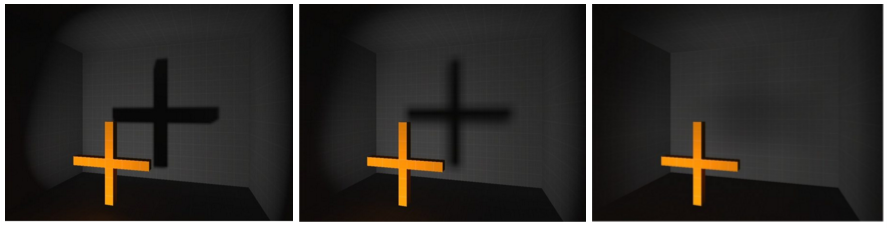
\includegraphics[width=0.8\linewidth]{images/chapter_stato_arte/stato_arte_scale_shadow.png}\hfill
 \caption[Fattore scala lumel]{Effetto dell'aumento del fattore scala dei lumel sulla risoluzione dell'ombra (da sinistra verso destra).}
 \label{fig:stato_arte_scale_shadow}
\end{figure}

Diminuendo il fattore scala aumenta la definizione della lightmap ma aumenta anche lo spazio occupato in memoria, peggiorando le prestazioni del rendering; per questo i grafici 3D spesso devono giungere a compromessi tra performance e qualità. Il mapping di una lightmap o di una texture, su di una superficie 3D avviene nello stesso modo: il processo, detto di texturizzazione, inizia individuando un punto nello spazio definito in coordinate modello; si sceglie questo sistema di riferimento in modo che la texture rimanga mappata sulla superficie sempre nello stesso modo, anche se la superficie si dovesse spostare. Dopodichè il vettore con le tre coordinate del punto viene proiettato in un vettore a due coordinate (u,v), avente ognuna un valore compreso nell’intervallo tra 0 e 1. Questi due valori sono moltiplicati per la risoluzione della texture, o della lightmap, ottenendo così la posizione del texel, o lumel, da mappare sul punto individuato nello spazio del modello.
\\
\begin{figure}[htb]
 \centering
 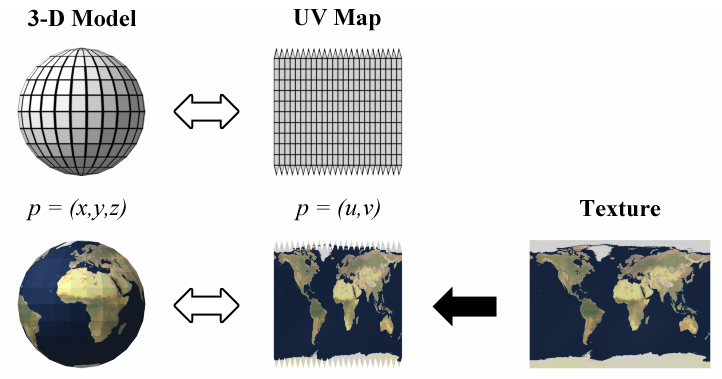
\includegraphics[width=0.8\linewidth]{images/chapter_stato_arte/stato_arte_uvmap.png}\hfill
 \caption[Texturizzazione mediante mappa UV]{Processo di texturizzazione di un oggetto.}
 \label{fig:stato_arte_uvmap}
\end{figure}

Quando viene creata una lightmap per ogni oggetto della scena, tipicamente ogni oggetto avra due texture: una texture diffuse che definisce il colore principale della superficie 3D, ed una lightmap con i valori di luce e ombra proiettati sull’oggetto della scena; quest’ultime tipicamente sono in bianco e nero, a meno che non vi sia del colore proveniente dalla luce stessa, o da un oggetto riflettente. 

Per ogni oggetto è possibile sommare lightmap e diffuse texture, moltiplicando i valori di irradianza della lightmap per i valori RGB della diffuse texture; in questo modo è possibile memorizzare un unica texture al posto di due. Anche se dal punto di vista del consumo di memoria è una soluzione vantaggiosa, ci sono comunque degli aspetti per cui vale la pena tenere separate le due mappe, primo fra tutti la riusabilità della diffuse texture.
Questa infatti è decisamente più riusabile di una lightmap, ad esempio è possibile ripetere una diffuse texture su di una superficie 3D. Sommando la diffuse ad una lightmap si perderebbe questo vantaggio. Inoltre in presenza di due scene identiche, una vista di giorno, l’altra di notte, è possibile generare due lightmap diverse mantenendo la stessa diffuse map.
\\
\begin{figure}[htb]
 \centering
 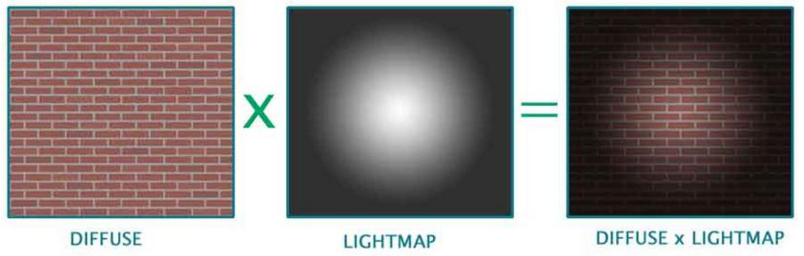
\includegraphics[width=0.8\linewidth]{images/chapter_stato_arte/stato_arte_diffuse_lightmap.png}\hfill
 \caption[Combinazione texture/lightmap]{Combinazione di una diffuse texture con una lightmap.}
 \label{fig:stato_arte_diffuse_lightmap}
\end{figure}

\subsection{Baking delle lightmap}
\label{sec:chapter_stato_arte_baking_lightmap}

Il processo di precomputazione delle informazioni di luce all’interno di una scena con oggetti e luci statiche, e la memorizzazione dei risultati all’interno di una struttura dati del tipo sopra descritto, è detto baking delle lightmap. Questo approccio è il migliore se si vogliono sfruttare algoritmi di illuminazione indiretta nelle applicazioni real-time, come i videogiochi. In generale, il baking delle lightmap porta in dote tutta una serie di vantaggi.
A livello qualitativo, il bake permette la fruizione di:
\begin{itemize}
\item Illuminazione indiretta.
\item Rimbalzi multipli.
\item Migliore illuminazione diretta.
\item Una più ampia scelta di sorgenti luminose da inserire nella scena.
\end{itemize}
Per quanto riguarda le performance:
\begin{itemize}
\item Sono elevate a tempo di esecuzione.
\item Non dipendono dal tipo di luce utilizzata.
\item Non dipendono dall’ algoritmo di illuminazione indiretta utilizzato.
\item Sono identiche sia per lightmap di ottima qualità, che di pessima qualità.
\item Permettono di aggiungere alla scena le sorgenti luminose che si desidera.
\item Sono scalabili.
\item Se si eseguisse l’algoritmo in realtime l’angolazione e la posizione delle luci, nonchè la posizione dell’osservatore, inficierebbero sule performance di rendering delle ombre e degli effetti di luce sulla scena.
\end{itemize}
L’intero processo di baking di una lightmap si può scomporre in tre fasi.

La prima fase riguarda il calcolo delle coordinate di texture della lightmap.
In questa fase il modello 2D della lightmap viene proiettato sulla superficie 3D del modello, individuando per ogni poligono della superficie una specifica area della lightmap.
Il processo di mappatura di una texture 2D su una superficie 3D è detto UV mapping.
\\
\begin{figure}[htb]
 \centering
 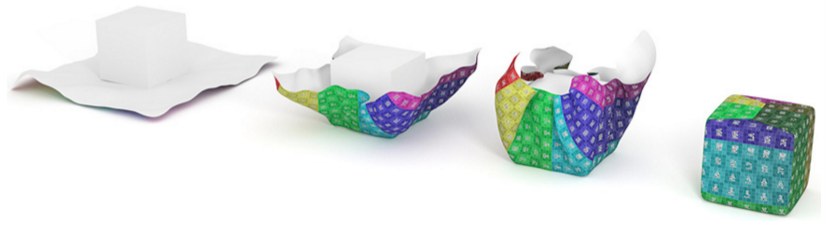
\includegraphics[width=0.8\linewidth]{images/chapter_stato_arte/stato_arte_unwrap.png}\hfill
 \caption[Mappatura delle coordinate UV]{Processo di unwrap (da destra verso sinistra).}
 \label{fig:stato_arte_unwrap}
\end{figure}

Si consideri il seguente esempio per comprendere il processo di UV Mapping.
Si supponga di avere uno scatolone, che può essere visto come un’ oggetto cubico 3D all’interno della scena. Aprendo lo scatolone in tutti i punti dove presenta una piega, si ottiene una superficie piana (Fig \ref{fig:stato_arte_unwrap}); questa procedura è detta \emph{unwrap} di un oggetto 3D su di un immagine 2D. Guardando questa superficie si definisce U la direzione destra o sinistra sulla superficie, e V la direzione in alto o in basso sulla stessa. Questa superficie viene definita \emph{mappa UV}. U e V sono dette coordinate di texture; (u=0,v=0) indica l’angolo in basso a sinistra della texture, mentre (u=1,v=1) indica l’angolo in alto a destra della stessa. Queste coordinate vengono usate al posto della X e Y che invece, insieme alla Z, fanno riferimento alle coordinate nello spazio 3D. Una volta riassemblata la scatola, una qualsiasi posizione (u,v) presente sulla superficie 2D, viene trasformata in una posizione (x,y,z) sulla scatola; questa operazione è detta wrap di un immagine 2D su di un oggetto 3D, e verrà descritto al passo successivo.

Una mappa UV può essere generata dall’applicazione software in modo completamente automatico, semi automatico, o creata a mano dall’artista 3D. Ad esempio utilizzando Blender, 
un software per la computer grafica 3D che verrà esposto in un paragrafo dedicato in quanto punto cardine del presente lavoro di tesi, espone un interfaccia per mezzo della quale poter decidere esattamente come mappare le facce di un oggetto 3D in un immagine 2D. 
\\
\begin{figure}[htb]
 \centering
 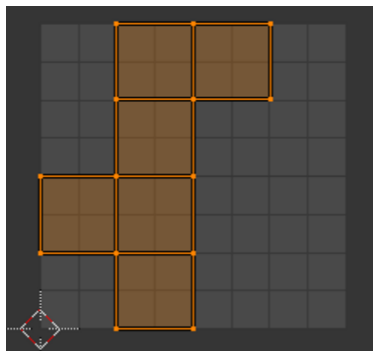
\includegraphics[width=0.5\linewidth]{images/chapter_stato_arte/stato_arte_uvmap_blender.png}\hfill
 \caption[Mappa UV realizzata in Blender]{Una mappa UV realizzata con il software di grafica 3D Blender.}
 \label{fig:stato_arte_uvmap_blender}
\end{figure}

Questa prima fase è fondamentale, perchè senza eseguire l’unwrap dell’oggetto 3D sulla lightmap è impossibile stabilire, dato il valore di radianza di un poligono dell’oggetto 3D, qual’è il lumel corrispondente in cui memorizzarlo.

La seconda fase prevede di calcolare la posizione in coordinate mondo e la normale, per ogni lumel in ogni lightmap.
Ogni lumel di una lightmap deve essere mappato in una posizione nel sistema di riferimento in coordinate mondo. Finchè le geometrie nella scena rimarrano statiche, e la dimensione delle lightmap rimarrà invariata, le corrispondenze tra coordinate texture e coordinate mondo risulteranno invariate, e quindi possono essere preprocessate offline una volta sola e poi riutilizzate.
A questo punto verrà mostrato come, partendo da una mappa UV di un poligono, le posizioni in coordinate texture vengono mappate in posizioni sulla superficie del poligono.
Si consideri il triangolo in figura \ref{fig:stato_arte_ligh_triangle1}: 
\\
\begin{figure}[htb]
 \centering
 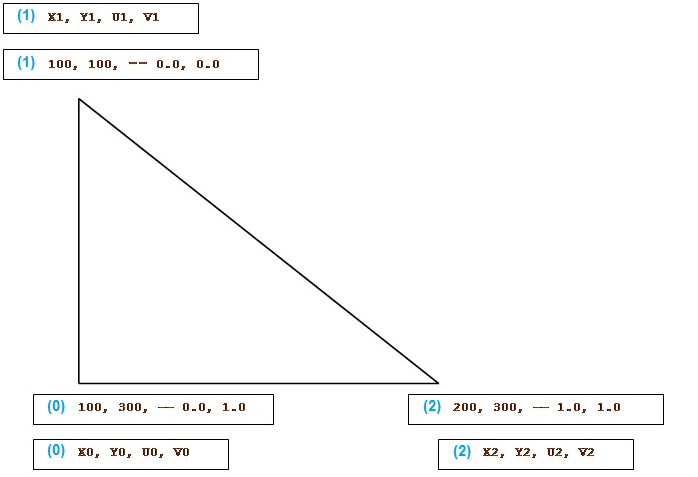
\includegraphics[width=1\linewidth]{images/chapter_stato_arte/stato_arte_ligh_triangle1.png}\hfill
 \caption[Triangolo di esempio per mapping UV]{Un triangolo definito all'interno di una mappa UV}
 \label{fig:stato_arte_ligh_triangle1}
\end{figure}

Come si può notare le componenti per la posizione dei vertici sono vettori 2D e non 3D; il motivo verrà spiegato più avanti.
Allo stato attuale i dati in possesso sono:	
\begin{itemize}
\item Le posizioni dei vertici del triangolo nel mondo.
\item Le coordinate texture $(u,v)$ per ognuno dei tre vertici.
\end{itemize}
Dato un punto in coordinate texture interno al poligono in figura \ref{fig:stato_arte_ligh_triangle1}, bisogna ottenere la posizione 2D del triangolo corrispondente nel mondo.
Un modo possibile è sfruttare le derivate per calcolare la variazione delle coordinate mondo $x$ e $y$ in base a come variano le coordinate texture $u$ e $v$; siccome in tutto sono 4 coordinate avremo 4 equazioni così espresse, in base ai vertici del triangolo in figura \ref{fig:stato_arte_ligh_triangle1}:
\\
\begin{equation}
\frac{dx}{du} = \frac{(x_1 - x_2)*(v_0 - v_2) - (x_0 - x_2)*(v_1 - v_2)}{(v_0 - v_2)*(u_1 - u_2) - (v_1 - v_2)*(u_0 - u_2)}
\label{dxdu}
\end{equation}
\begin{equation}
\frac{dx}{dv} = \frac{(x_1 - x_2)*(u_0 - u_2) - (x_0 - x_2)*(u_1 - u_2)}{(v_0 - v_2)*(u_1 - u_2) - (v_1 - v_2)*(u_0 - u_2)}
\label{dxdv} 
\end{equation}
\begin{equation}
\frac{dy}{du} = \frac{(y_1 - y_2)*(v_0 - v_2) - (y_0 - y_2)*(v_1 - v_2)}{(v_0 - v_2)*(u_1 - u_2) - (v_1 - v_2)*(u_0 - u_2)}
\label{dydu}
\end{equation}
\begin{equation}
\frac{dy}{dv} = \frac{(y_1 - y_2)*(u_0 - u_2) - (y_0 - y_2)*(u_1 - u_2)}{(v_0 - v_2)*(u_1 - u_2) - (v_1 - v_2)*(u_0 - u_2)} 
\label{dydv}
\end{equation}
Per la derivazione completa delle quattro equazioni si rimanda a [numero fonte], tuttavia l’idea di base è piuttosto semplice. Osservando la figura \ref{fig:stato_arte_ligh_triangle2} si supponga di dover determinare come varia la coordinata $x$ rispetto alla $u$. Per fare questo si fissa la coordinata $v$ e si muove la $u$. Così facendo viene individuato un nuovo generico punto nello spazio. 
\\
\begin{figure}[htb]
 \centering
 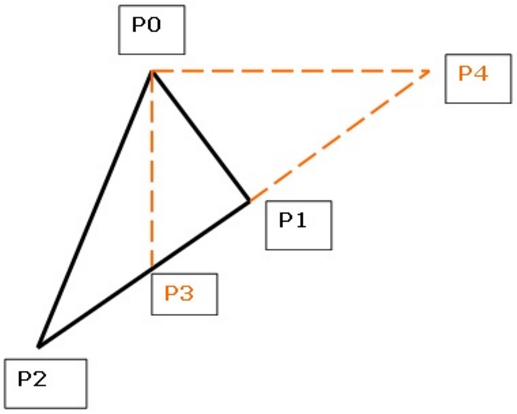
\includegraphics[width=0.5\linewidth]{images/chapter_stato_arte/stato_arte_ligh_triangle2.png}\hfill
 \caption[Triangolo di esempio per calcolo coordinate]{Dal vertice $p_0$ del triangolo in foto, si ottiene il punto $p_4$ mantenendo fissa la coordinata $v$ di $p_0$ e variando la coordinata $u$.}
 \label{fig:stato_arte_ligh_triangle2}
\end{figure}

Dalla figura \ref{fig:stato_arte_ligh_triangle2} si può vedere come, fissando la $v$ e muovendo $p_0$ lungo l’asse delle $u$, si ottiene il punto $p_4$. A questo punto viene calcolata la variazione di $x$ rispetto a $u$ nello spostamento da $p_0$ a $p_4$:
\begin{equation}
\frac{dx}{du} = \frac{(x_4 - x_0)}{(u_4 - u_0)} 
\label{derivata_1}
\end{equation}

Dall'equazione \ref{derivata_1} vengono quindi individuate due componenti: $dx = (x_4-x_0)$ dove l’incognita è $x_4$, e $du = (u_4-u_0)$ dove l’incognita è $u_4$ E’ possibile ottenere queste coordinate di $p_4$ utilizzando l’equazione della retta passante per due punti: costruendo il triangolo come in figura \ref{fig:stato_arte_ligh_triangle2}, la retta passante per $p_1$ e $p_2$ è la stessa che passa per $p_3$ e $p_4$, pertanto è possibile definire le equazioni per due rette: una usando $x_4$ come ingognita, e $x_1,x_2,y_1,y_2,y_4=y_0$ come coordinate note, e l’altra con $u_4$ come incognita e $u_1,u_2,v_1,v_2,v_4=v_0$ come coordinate note:
\begin{equation}
\frac{(x_1 - x_2)}{(y_1 - y_2)} = \frac{(x_4 - x_2)}{(y_4 - y_2)} 
\label{eq_retta1}
\end{equation}
\begin{equation}
\frac{(u_1 - u_2)}{(v_1 - v_2)} = \frac{(u_4 - u_2)}{(v_4 - v_2)} 
\label{eq_retta2}
\end{equation}

A questo punto l’ultimo passaggio consiste nell'esprimere l'equazione \ref{eq_retta1} in funzione di $x_4$, e l'equazione \ref{eq_retta2} in funzione di $u_4$, e sostituirle in \ref{derivata_1}; svolgendo i calcoli si arriva ad una forma equivalente alle equazioni \ref{dxdu},\ref{dxdv},\ref{dydu},\ref{dydv}. 
Ottenute le quattro equazioni manca un’ultimo un passaggio, ovvero calcolare lo spostamento di un generico punto $(u,v)$ della lightmap rispetto al primo vertice $(u_0,v_0)$:
\begin{equation}
s_u = u - u_0
\end{equation}
\begin{equation}
s_v = v - v_0
\end{equation}
Si hanno quindi tutti gli elementi per scrivere l’equazione della posizione finale $(x,y)$ corrispondente ad un punto $(u,y)$ in coordinate texture della lightmap:
\begin{equation}
x = x_0 + (\frac{d_x}{d_u} * s_u) + (\frac{d_x}{d_v} * s_v)
\label{eq_fin1}
\end{equation}
\begin{equation}
y = y_0 + (\frac{d_y}{d_u} * s_u) + (\frac{d_y}{d_u} * s_v)
\label{eq_fin2}
\end{equation}
Per ognuna di queste equazioni si calcolano, a partire dalla posizione del vertice iniziale, il comportamento di $x$ e $y$ al variare di $u$ e $v$ moltiplicato per lo spostamento effettivo sulle coordinate $u$ e $v$.

A questo punto è possibile ottenere la posizione $(x,y)$ corrispondente alle coordinate $(u,v)$; tuttavia  manca ancora un dettaglio: in una scena i poligoni appartengono ad oggetti definiti in uno spazio a tre dimensioni,quindi le rispettive posizioni devono essere definite in tre coordinate piuttosto che due. 
Per ottenere la terza coordinata di sfrutta l’equazione del piano. 
\begin{equation}
ax + by + cz = d
\label{eq_piano}
\end{equation}
Se ad esempio, per il calcolo delle equazioni \ref{eq_fin1} e \ref{eq_fin2} si utilizzasse come riferimento un triangolo proiettato sugli assi $x$ e $z$, e quindi mancante della coordinata $y$, tale coordinata potrebbe essere ricavata da \ref{eq_piano} nel modo seguente:
\begin{equation}
ax + by + cz = d
\end{equation}
\begin{equation}
by = -(ax + cz + d)
\end{equation}
\begin{equation}
y = - \frac{(ax + cz + d)}{b}
\end{equation}
Il procedimento è il medesimo se si volessero estrarre le componenenti X o Z.

La fase finale prendere il calcolo della componente RGB da associare ad ogni pixel.
Questo è l’ultimo processo coinvolto nel calcolo delle lightmap, dove viene assegnato un valore ad ogni lumel. A questo punto viene mostrata una descrizione in pseudocodice di come funziona un semplice l’algoritmo per il calcolo del colore per ogni lumel di una ligthmap:

\begin{itemize}
\item Sia L la lightmap (vista come matrice di lumels).
\item Sia H l'altezza della lightmap.
\item Sia W la larghezza della lightmap.
\item Siano I e J due indici per iterare gli elementi di L.
\end{itemize}
 
\begin{algorithm}[H]
 \For{I = 0; I < H; I++} {
  \For{J = 0; I < W; I++} { 
   Sia CL = L[I,J], ovvero il lumel corrente\;
   \For{ogni LI nella scena} {
    \If{LI guarda in una posizione diversa da dove si trova CL}
     {
     Ignora l'effetto di LI su CL e passa al lumel successivo\;
     }
	\If{La distanza tra CL e LI è maggiore del raggio d'azione di LI}
	 {
     Ignora l'effetto di LI su CL e passa al lumel successivo\;
     }
	\If{I primi due test hanno avuto esito positivo}
	 {
     N = numero di collisioni dei raggi da LI a CL\;
     }
	\If{N > 0}
	 {
     Estrai il colore da LI e memorizzalo in CL\;
     }
    }
   }
  }
\end{algorithm}

L’algoritmo gestisce per ogni lumel una struttura dati contenente:
\begin{itemize}
\item Posizione del lumel in coordinate mondo.
\item La normale del lumel.
\item Il colore finale.
\item Le componenti R,G.B e Alpha del colore.
\item Un booleano che indica se la posizione del lumel è valida, ovvero se il lumel appartiene a qualche poligono o meno.
\item Un riferimento al poligono di cui il lumel da parte. 
\end{itemize}
La dimensione di questa struttura dati determinerà la dimensione della lightmap; si supponga infatti che la struttura pesi 4 bytes, e che la lightmap abbia una risoluzione di 1024x1024, la dimensione totale sarà 1024*1024*4 = 4194304 bytes = 4 Mb. Ovviamente la quantità di memoria allocata per la struttura dati può essere considerevolmente ridotta, diminuendo lo spazio occupato dall’immagine.
I risultati dell’algoritmo per il calcolo del colore per ogni lumel possono essere ulteriormente processati per migliorarne la qualità.
Siccome senza l’applicazione di alcun filtro l’immagine finale potrebbe apparire sgranata, si potrebbe migliorare l’esperienza visiva applicando dei filtri. 
Ad esempio si potrebbe ridurre il distacco di colore tra un pixel e l’adiacente aggiungendo un effetto blur; l’algoritmo per l’applicazione di un effetto di questo tipo è molto semplice:


\begin{itemize}
\item Sia L la lightmap (vista come matrice di lumels).
\item Sia H l'altezza della lightmap.
\item Sia W la larghezza della lightmap.
\item Siano I e J due indici per iterare gli elementi di L.
\end{itemize}
 
\begin{algorithm}[H]
 \For{I = 0; I < H; I++} {
  \For{J = 0; I < W; I++} { 
    Sia CL = L[I,J], ovvero il lumel corrente\;
    Sia S la somma degli 8 lumel confinanti con CL, ignorando i lumel non validi\;
    Sia A = S/numero dei lumel validi confinanti con CL\;
    Aggiornare il valore in L[I,J] con A\;
   }
  }
\end{algorithm}

\subsection{Contesto di utilizzo}
\label{sec:chapter_stato_arte_contex_use}

Gli algoritmi di illuminazione globale, o indiretta, sono onerosi dal punto di vista computazionale, specialmente per il rendering in real-time. 
Tuttavia in una scena statica, o parzialmente statica, l’illuminazione indiretta può essere pre-processata, memorizzando i risultati per utilizzarli durante il rendering. 
I rimbalzi multipli di luce su delle superfici creano giochi di luci e ombre che sono alla base di una scena realistica. Le interriflessioni portano inoltre al fenomeno del color blending, dove il colore di un oggetto appare su un oggetto adiacente. 
Radiosity è stata la prima tecnica nella computer grafica a simulare i rimbalzi di luce tra superfici diffuse. 
L’idea alla base di questo algoritmo è relativamente semplice. Se in un ambiente viene accesa una luce, le particelle luminose cominceranno a rimbalzare per tutto l’ambiente, fino a raggiungere una condizione di equilibrio. In questa condizione di equilibrio, la superficie può essere considerata essa stessa una fonte luminosa. 
Una superficie colpita da una fonte luminosa può assorbire o riflettere la luce stessa. L’algoritmo radiosity pone dapprima l’assunzione base che tutte le luci indirette provengono da superfici diffuse: una tesi questa che crolla nel momento in cui si ha a che fare ad esempio con un pavimento di marmo lucido, o uno specchio, ma in generale per la maggior parte degli ambienti può rivelarsi una buona approssimazione. Basandosi su questa tesi, la funzione di distribuzione bidirezionale della riflettanza (BRDF) per superfici diffuse, ovvero la funzione che regola come la luce viene riflessa su di una superficie opaca, è una semisfera uniforme.
\\
\begin{figure}[htb]
 \centering
 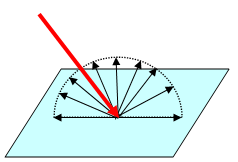
\includegraphics[width=0.5\linewidth]{images/chapter_stato_arte/stato_attuale_brdf_semistefa.png}\hfill
 \caption[BRDF superfici diffuse]{BRDF per superfici diffuse}
 \label{fig:stato_attuale_brdf_semistefa}
\end{figure}
Quindi la quantità di radiazione luminosa emessa della superficie (radianza) è proporzionale al flusso di radiazione luminosa incidente la superficie (irradianza) moltiplicato per il potere riflettente della superficie. 
\begin{equation}
L_s = \frac{r*E}{\pi}
\end{equation}
L’algoritmo prevede che ad ogni superficie ne corrisponda una analoga rappresentata da dei poligoni; non è necessario che ci sia una relazione 1:1 con i poligoni della superficie originale, infatti è possibile utilizzarne anche meno, o di più in caso si volesse un maggior dettaglio delle ombre. 
A questo punto viene creata una matrice di fattori forma con tutti i poligoni utilizzati. Questa matrice, dato un poligono i e un poligono j, restituisce il fattore forma Fij, ovvero un valore geometrico che denota una proporzione della quantità di luce che, partendo dal poligono i, arriva al poligono j. 
Una parte significativa dell’algoritmo radiosity è dedicata a calcolare in modo accurato i fattori forma tra tutti i poligoni della scena. 
Il fattore forma Fij dipende dai seguenti parametri:
\begin{itemize}
\item La forma dei due poligoni i e j.
\item L’orientamento dei due poligoni.
\item La distanza tra i e j.
\item L’occlusione di i e j a causa di altri poligoni.
\end{itemize}
Una volta ottenute tutte le relazioni geometriche tra i poligoni, alcuni poligoni sono designati come fonti luminose; questa designazione è necessaria per i processamenti al passo successivo. 
Come gia menzionato, le radiazioni luminose pervadono la scena fino ad ottenere una situazione di equilibrio; per calcolare questo equilibrio, l’algoritmo risolve un complesso sistema di equazioni lineari (riferimento bibliografico libro).
Risolvendo questo sistema di equazioni lineari si ottengono i valori di radianza per ogni poligono, e quindi la radianza di tutta la superficie; questo avviene perchè la radianza nelle superfici diffuse è costante e non dipende dall’angolo di vista.
La parte computazionalmente più onerosa è la risoluzione del sistema di equazioni lineari, e nonostante le GPU diventino sempre più veloci, il calcolo di alcuni algoritmi rimane tuttavia proibitivo per le applicazioni che necessitano di rendering real-time. 
Pertanto il calcolo dell’algoritmo radiosity viene fatto off-line, e le risultanti informazioni luminose possono essere memorizzate sui vertici delle superifici e poi interpolate, oppure memorizzate su delle lightmap per ogni superficie. 
In questo modo durante il ciclo di rendering, nella fase calcolo dello shading sui vertici delle geometrie, non sarà necessaria alcuna computazione delle informazioni di luce. 
\\
\begin{figure}[htb]
 \centering
 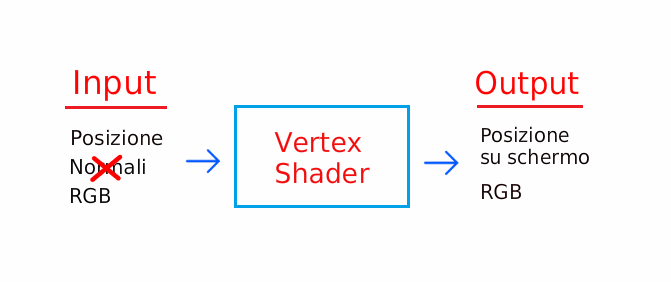
\includegraphics[width=0.8\linewidth]{images/chapter_stato_arte/stato_arte_ver_sh.jpg}\hfill
 \caption[Vertex shading lightmap]{Dettaglio circa l'operazioni di vertex shading utilizzando le lightmap.}
 \label{fig:stato_arte_ver_sh}
\end{figure}

La Id Software nel 1997 fu la prima 
software house che, per la realizzazione del videogioco Quake II, processò offline l’algoritmo radiosity, memorizzando le informazioni di luce su delle lightmap.
\\
\begin{figure}[htb]
 \centering
 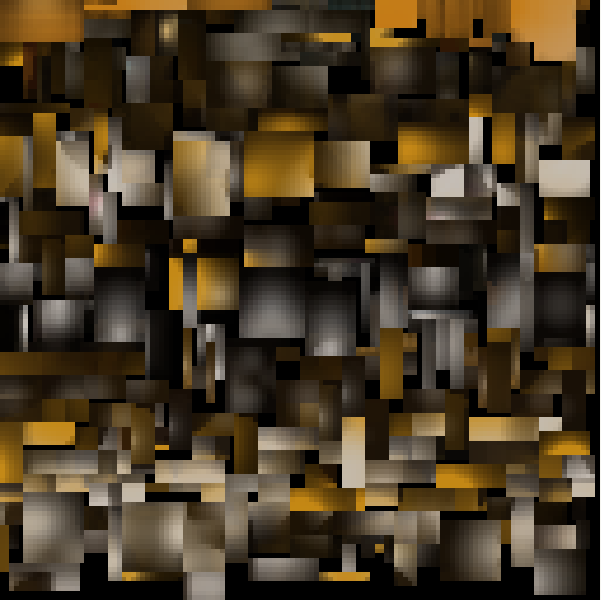
\includegraphics[width=0.5\linewidth]{images/chapter_stato_arte/stato_arte_quake_lightmap.png}\hfill
 \caption[Lightmap Quake II]{Una lightmap utilizzata nel videogioco Quake II (1997).}
 \label{fig:stato_arte_quake_lightmap}
\end{figure}

Nonostante gli anni, il pre-calcolo offline delle luci rimane una tecnica attuale; ne è la prova The Witness, un gioco di avventura con elementi puzzle sviluppato da Thekla e uscito il 26 
gennaio 2016. Per lo stile grafico dell’opera l’autore Jonathan Blow vide l’illuminazione indiretta come soluzione migliore, in modo da poter simulare i rimbalzi di luce attraverso la scena ed ottenere un aspetto più ricco e delicato rispetto a soluzioni come quelle adottate generalmente dagli shooter in prima persona, dove si fa largo uso di illuminazione diretta, ombre dinamiche, ed effetti particellari. Siccome calcolare la luce indiretta in tempo reale sarebbe stato troppo gravoso, la soluzione finale fu quella di pre-computarla e mappare i risultati su delle   lightmap.	
\\
\begin{figure}[htb]
 \centering
 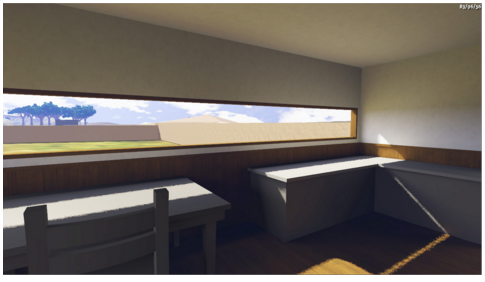
\includegraphics[width=0.8\linewidth]{images/chapter_stato_arte/stato_arte_lightmap_witness.png}\hfill
 \caption[Lightmap The Witness]{Un ambiente alpha con luci precomputate, tratto dal videogioco The Witness (2016)}
 \label{fig:stato_arte_lightmap_witness}
\end{figure}
